\documentclass[12pt]{article}
\usepackage[english]{babel}
\usepackage{amsmath,amsthm,amsfonts,amssymb,epsfig}
\usepackage[left=.5in,top=.5in,right=.5in, bottom=1in]{geometry}
\usepackage{mathtools}
\usepackage{breqn}



\usepackage{titlesec}
\usepackage{verbatim}
\usepackage{amssymb}
\usepackage{amsmath}
\usepackage{amsthm}
\usepackage{mathrsfs}
\usepackage{enumitem}

\usepackage{graphicx}

%% commands for math note taking 
\newcommand{\defn} [0]  {\paragraph{DEFN : }}
\newcommand{\fact}[0] {\paragraph{FACT : }}
\newcommand{\prop} [0] {\paragraph{PROP  : }}
\newcommand{\thm}[0] {\paragraph{THM : }}
\newcommand{\cor}[0] {\paragraph{COROLLARY : }}
\newcommand{\pf}[0] {\paragraph*{PROOF :}}
\newcommand{\note}[0] {\paragraph*{NOTE :}}
\newcommand{\lemma}[0]{\paragraph*{LEMMA : }}
\DeclarePairedDelimiter{\abs}{\lvert}{\rvert}


\newcommand*{\backnotin}{\rotatebox[origin=c]{-180}{$\notin$}}%

\titleformat{\subsection}{\centering\large\bfseries}{\thesection}{1em}{}



\DeclareMathOperator{\tr}{tr}
\DeclareMathOperator{\im}{im}
\DeclareMathOperator{\Perm}{Perm}
\DeclareMathOperator{\lcm}{lcm}
\DeclareMathOperator{\Var}{Var}
\DeclareMathOperator{\Cov}{Cov}

\title{Amazon Html Notes}
\author{Darek Johnson}
\date{Mar 4, 2017}

\begin{document}

%%  eliminates page numbers
%%  \pagestyle{empty}

\maketitle

\section*{}
For 2 amazon products with different page layouts we'll show some div tags of note. The section names are the div's id tag \\ \\

\begin{enumerate}
	\item https://www.amazon.com/dp/B01GKDYHGS/ (smart scale)
	\item https://www.amazon.com/dp/B00LGRY8AO/  (sweat pants)
\end{enumerate}

\pagebreak 

\section*{actionPanelContainer}
\begin{figure}[htp]
\centering
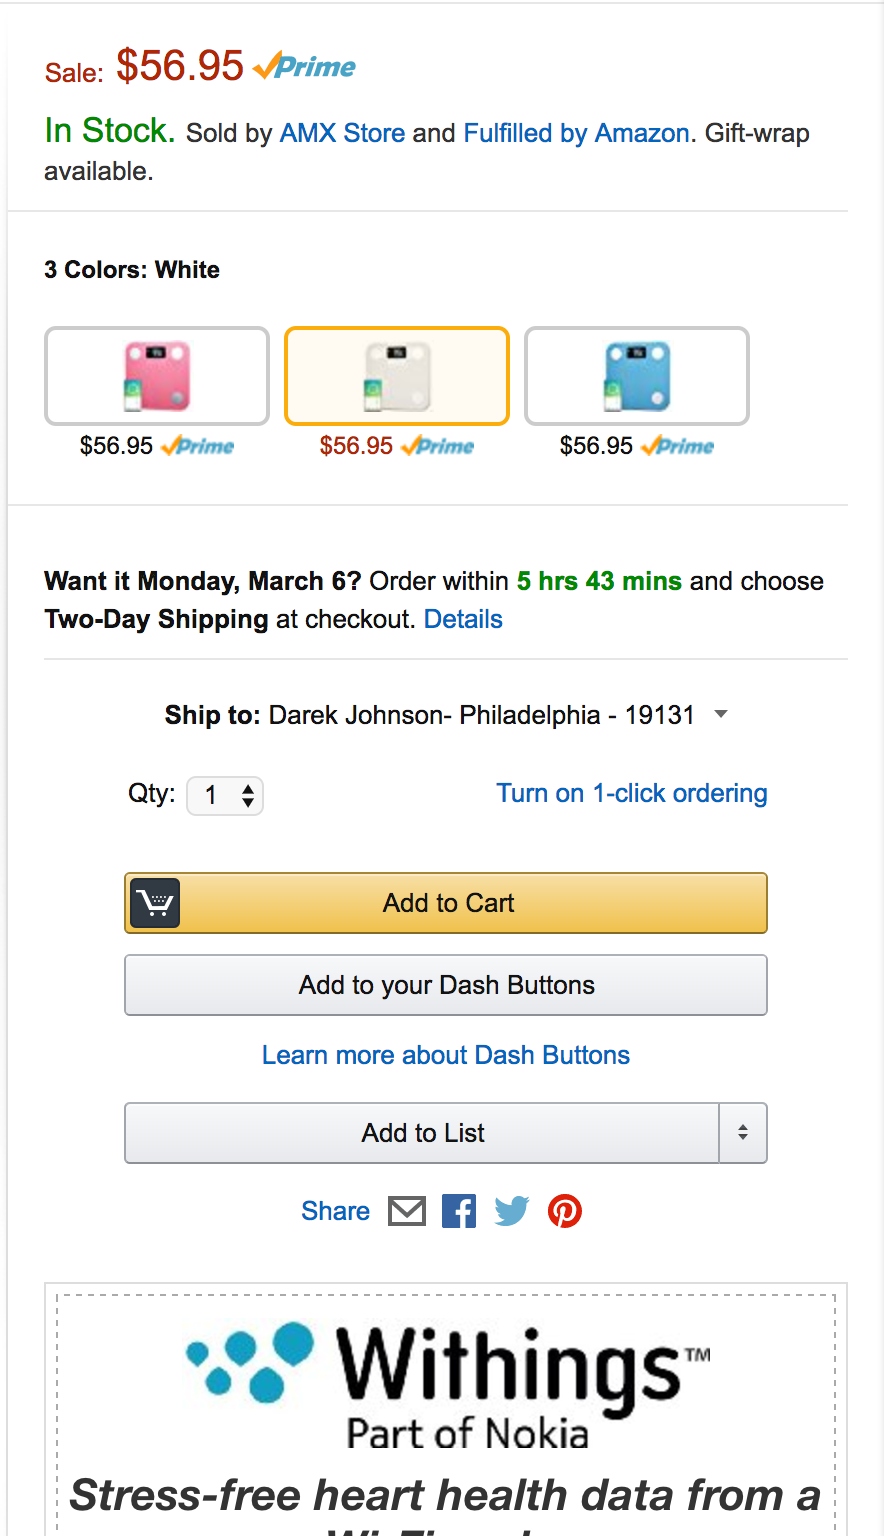
\includegraphics[width=300px,height=300px]{images/actionPanelContainer(1).png}
\caption{(1)}
\end{figure}


\pagebreak


\section*{centerCol}
\begin{figure}[htp]
\centering
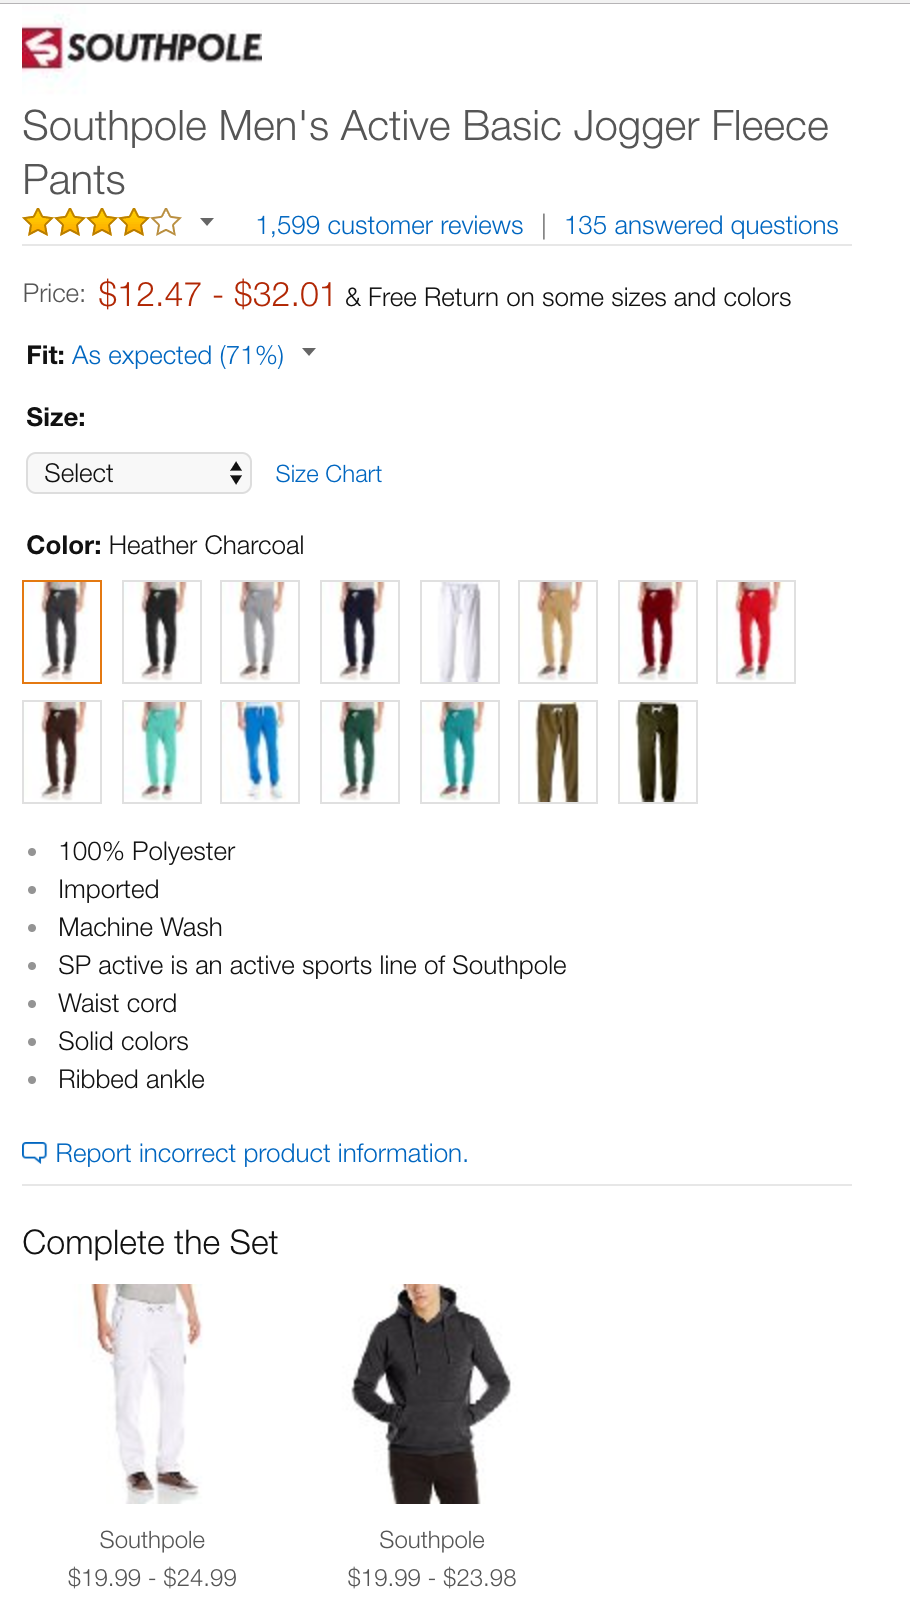
\includegraphics[width=300px,height=300px]{images/centerCol(2).png}
\caption{(2)}
\end{figure}

\pagebreak

\section*{descriptionAndDetails}
\begin{figure}[htp]
\centering
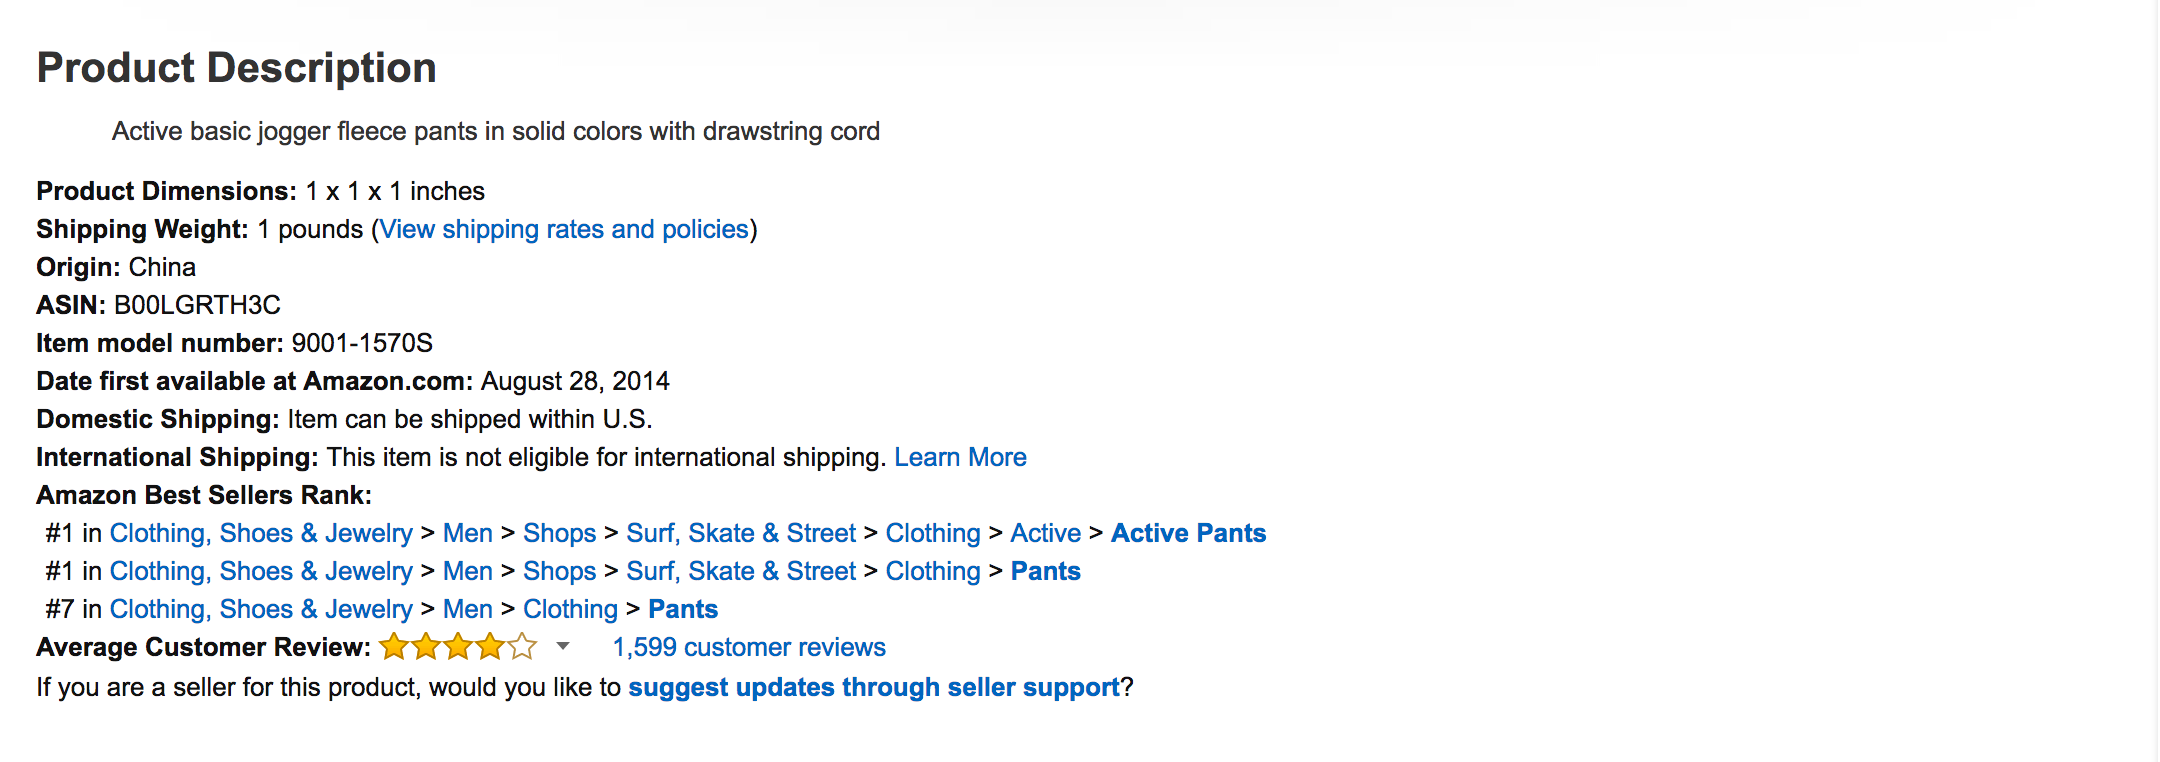
\includegraphics[width=300px,height=300px]{images/descriptionAndDetails(2).png}
\caption{(2)}
\end{figure}

\pagebreak
\section*{detail-bullets\_feature\_div}
\begin{figure}[htp]
\centering
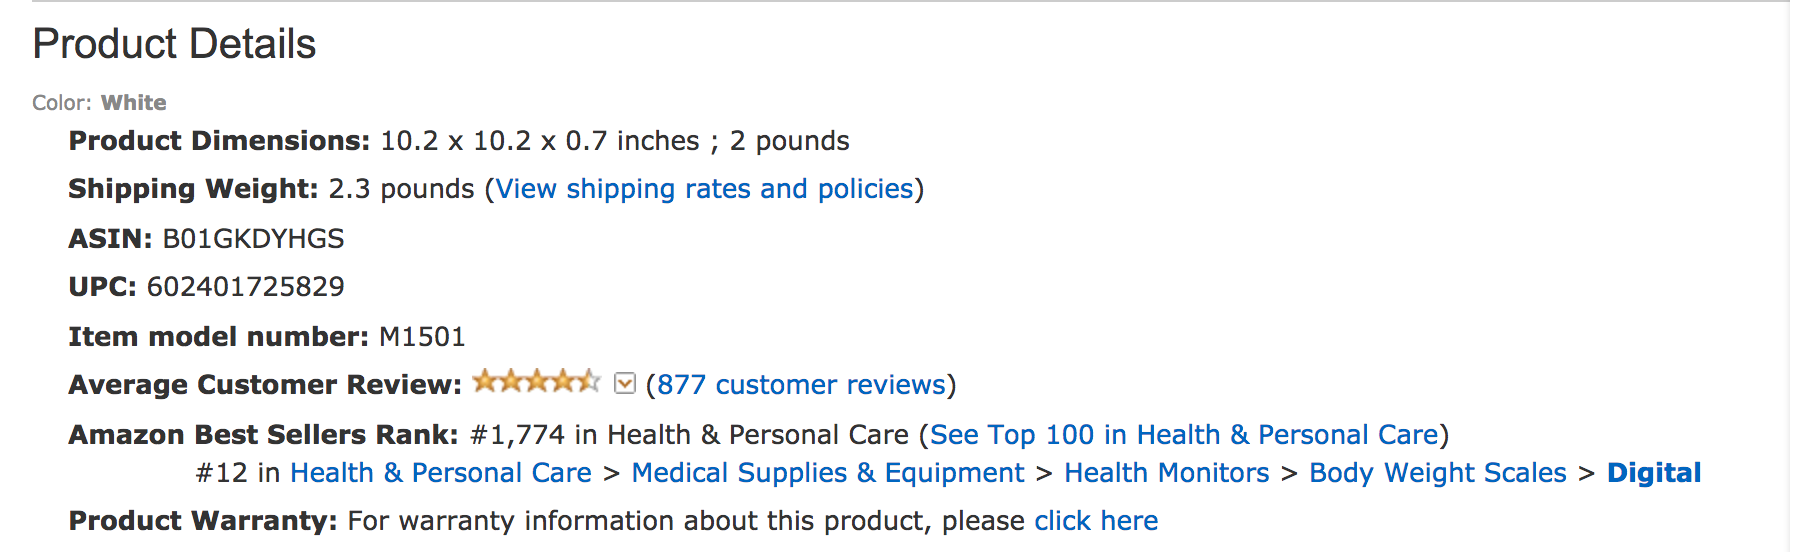
\includegraphics[width=300px,height=100px]{images/detail-bullets_feature_div(1).png}
\caption{(1)}
\end{figure}


\pagebreak
\section*{dpx-aplus-product-description\_feature\_div}
\begin{figure}[htp]
\centering
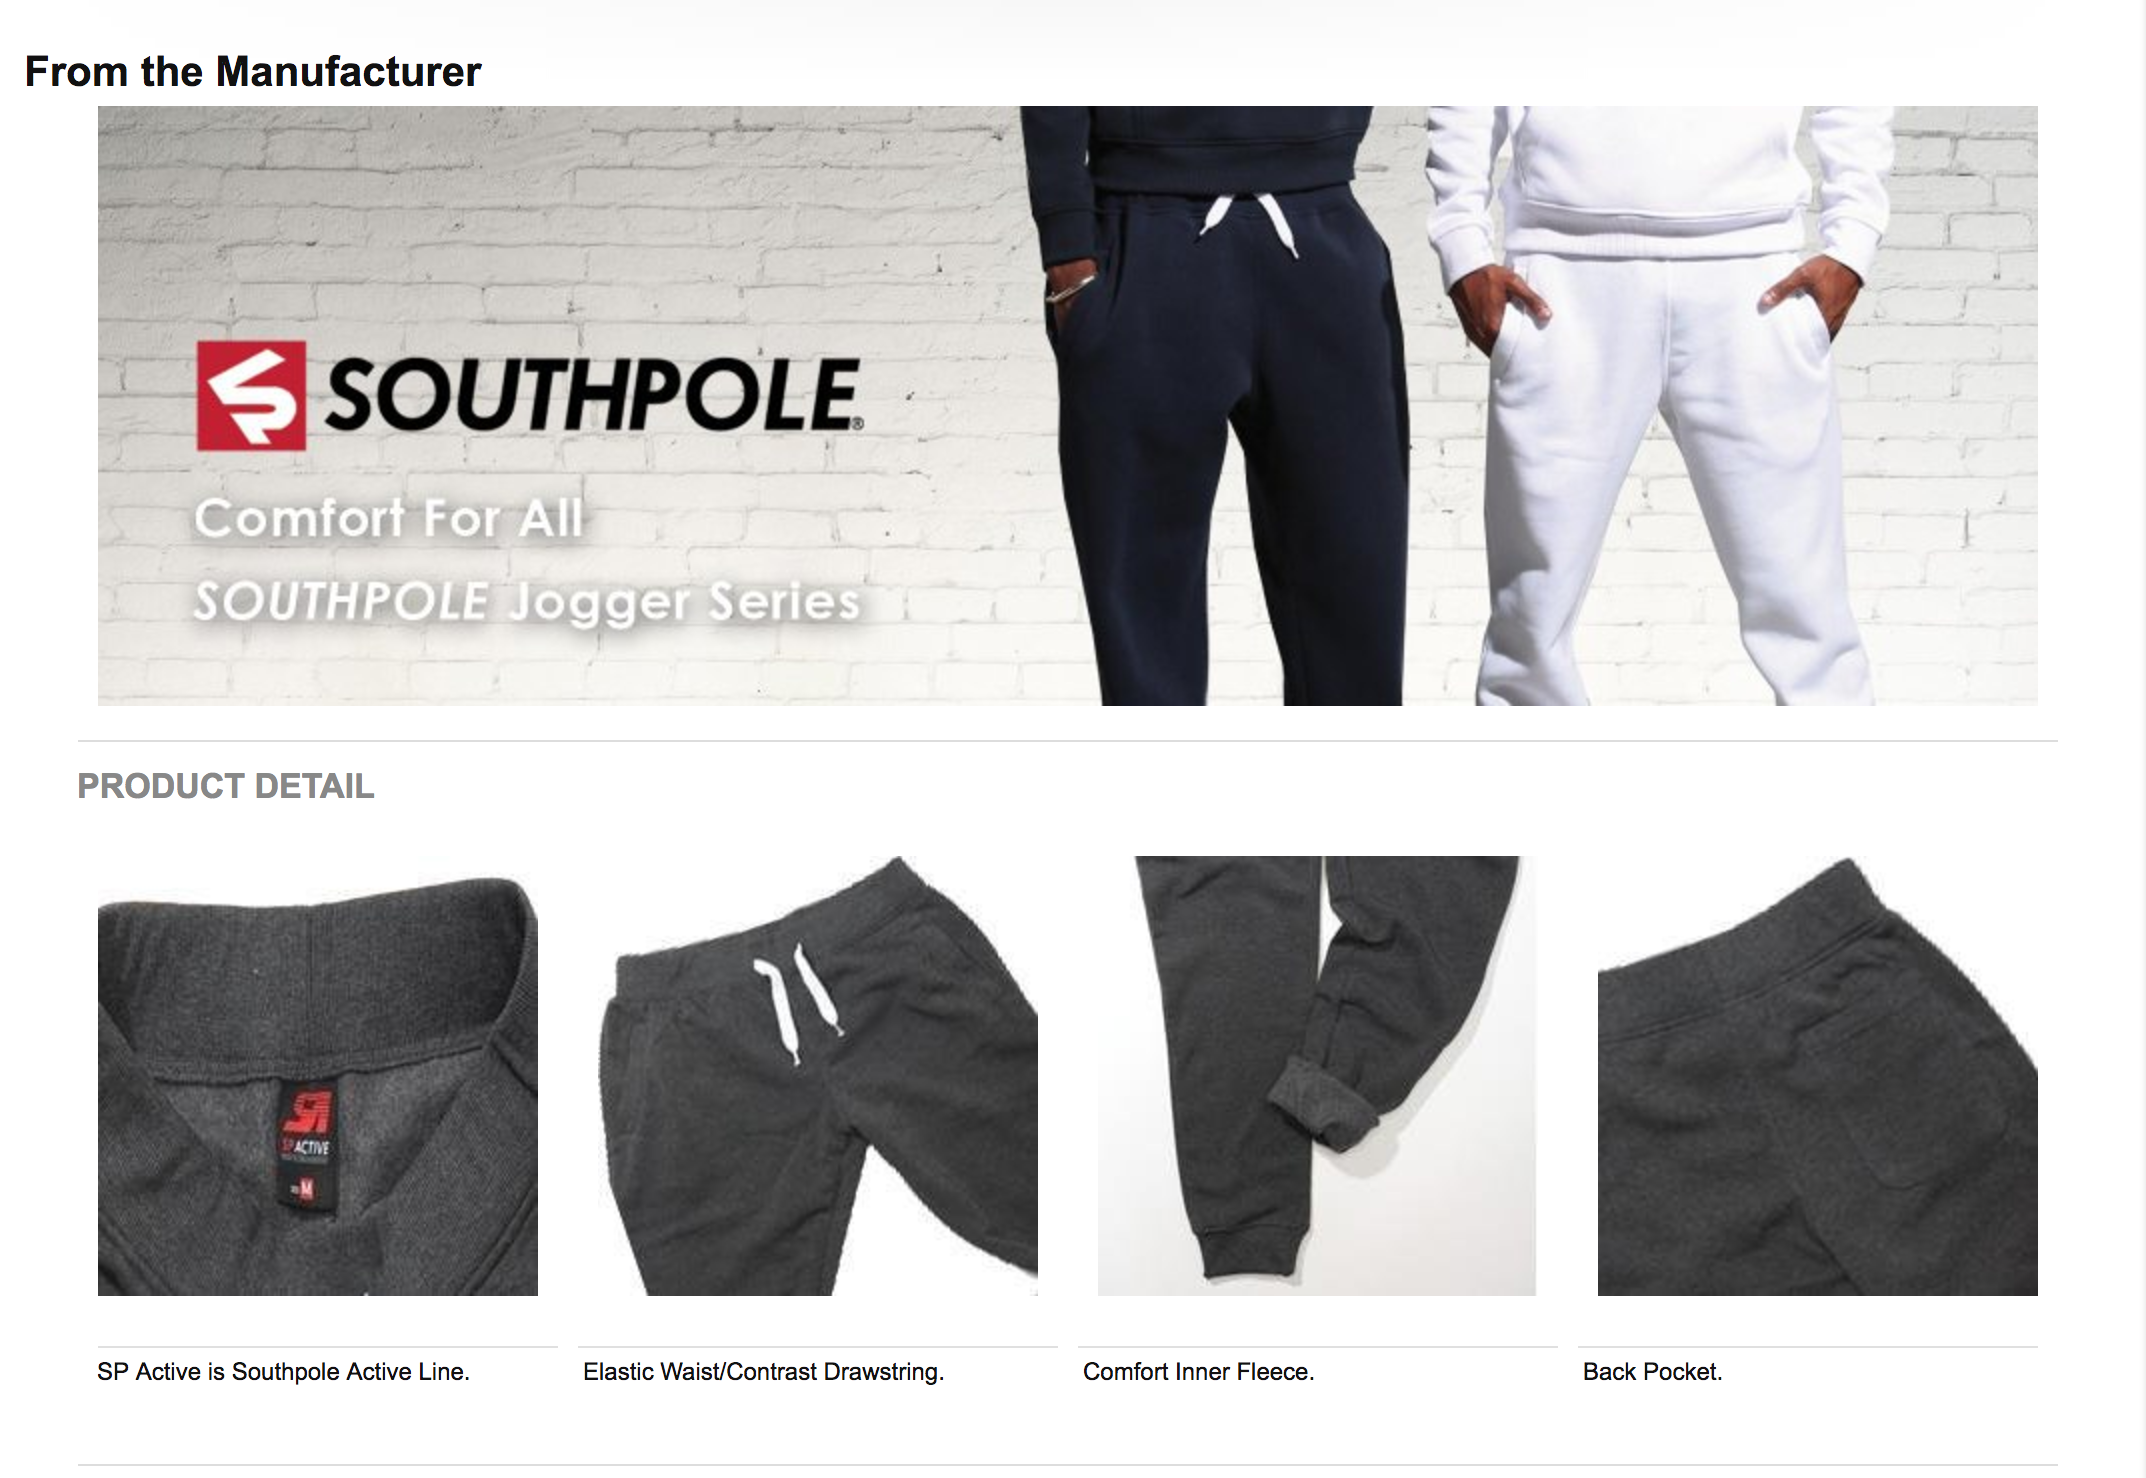
\includegraphics[width=300px,height=300px]{images/dpx-aplus-product-description_feature_div(2).png}
\caption{(1)}
\end{figure}


\pagebreak

\section*{sims-consolidated-1\_feature\_div}
\begin{figure}[htp]
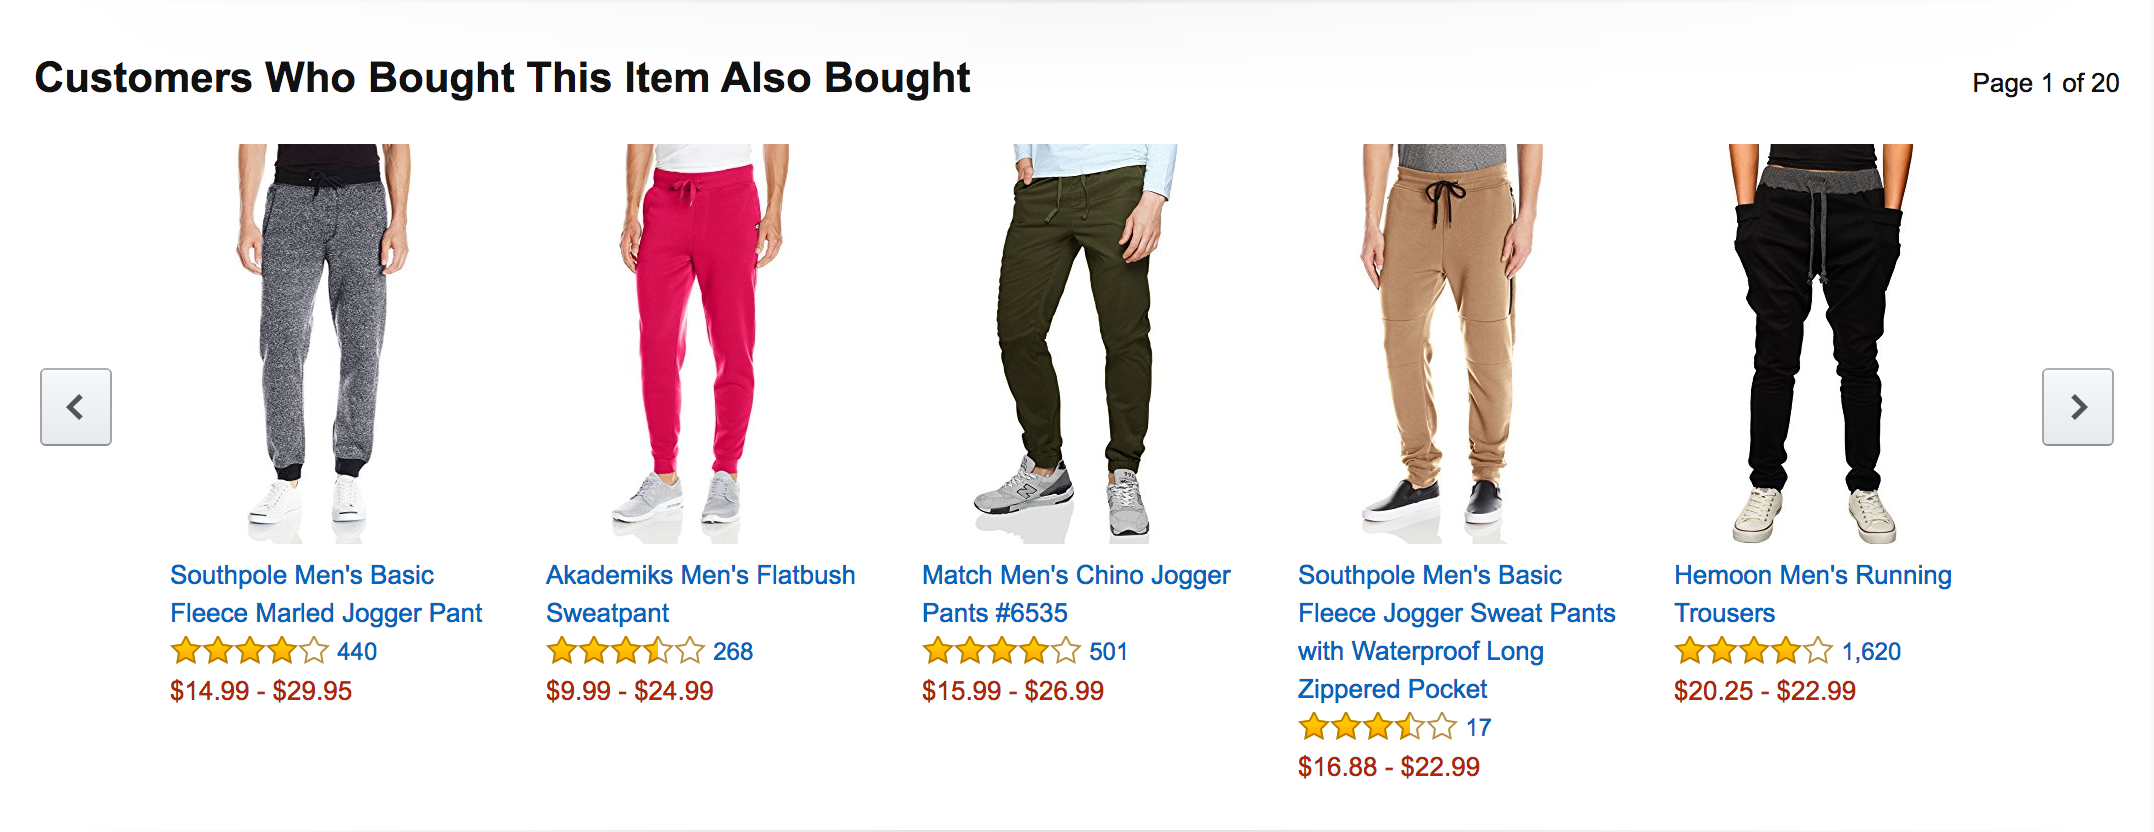
\includegraphics[width=300px,height=300px]{images/sims-consolidated-1_feature_div(2).png}
\caption{(2)}
\end{figure}

\pagebreak


\section*{sims-consolidated-2\_feature\_div}
\begin{figure}[htp]
\centering
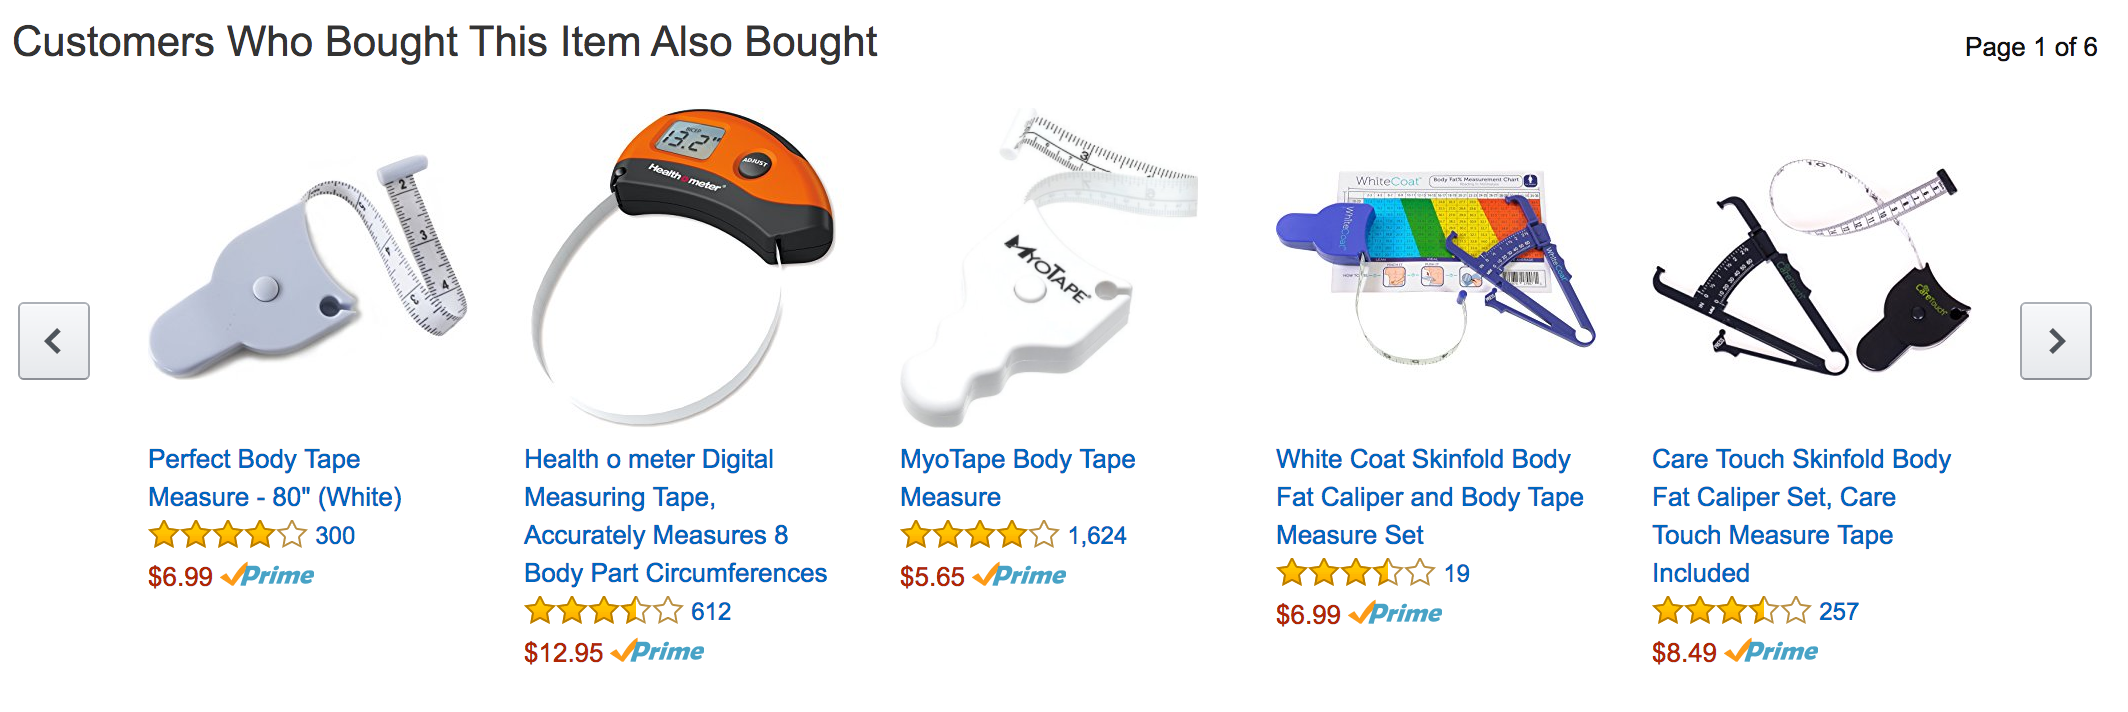
\includegraphics[width=300px,height=300px]{images/sims-consolidated-2_feature_div(1).png}
\caption{(1)}
\end{figure}
\begin{figure}[htp]
\centering
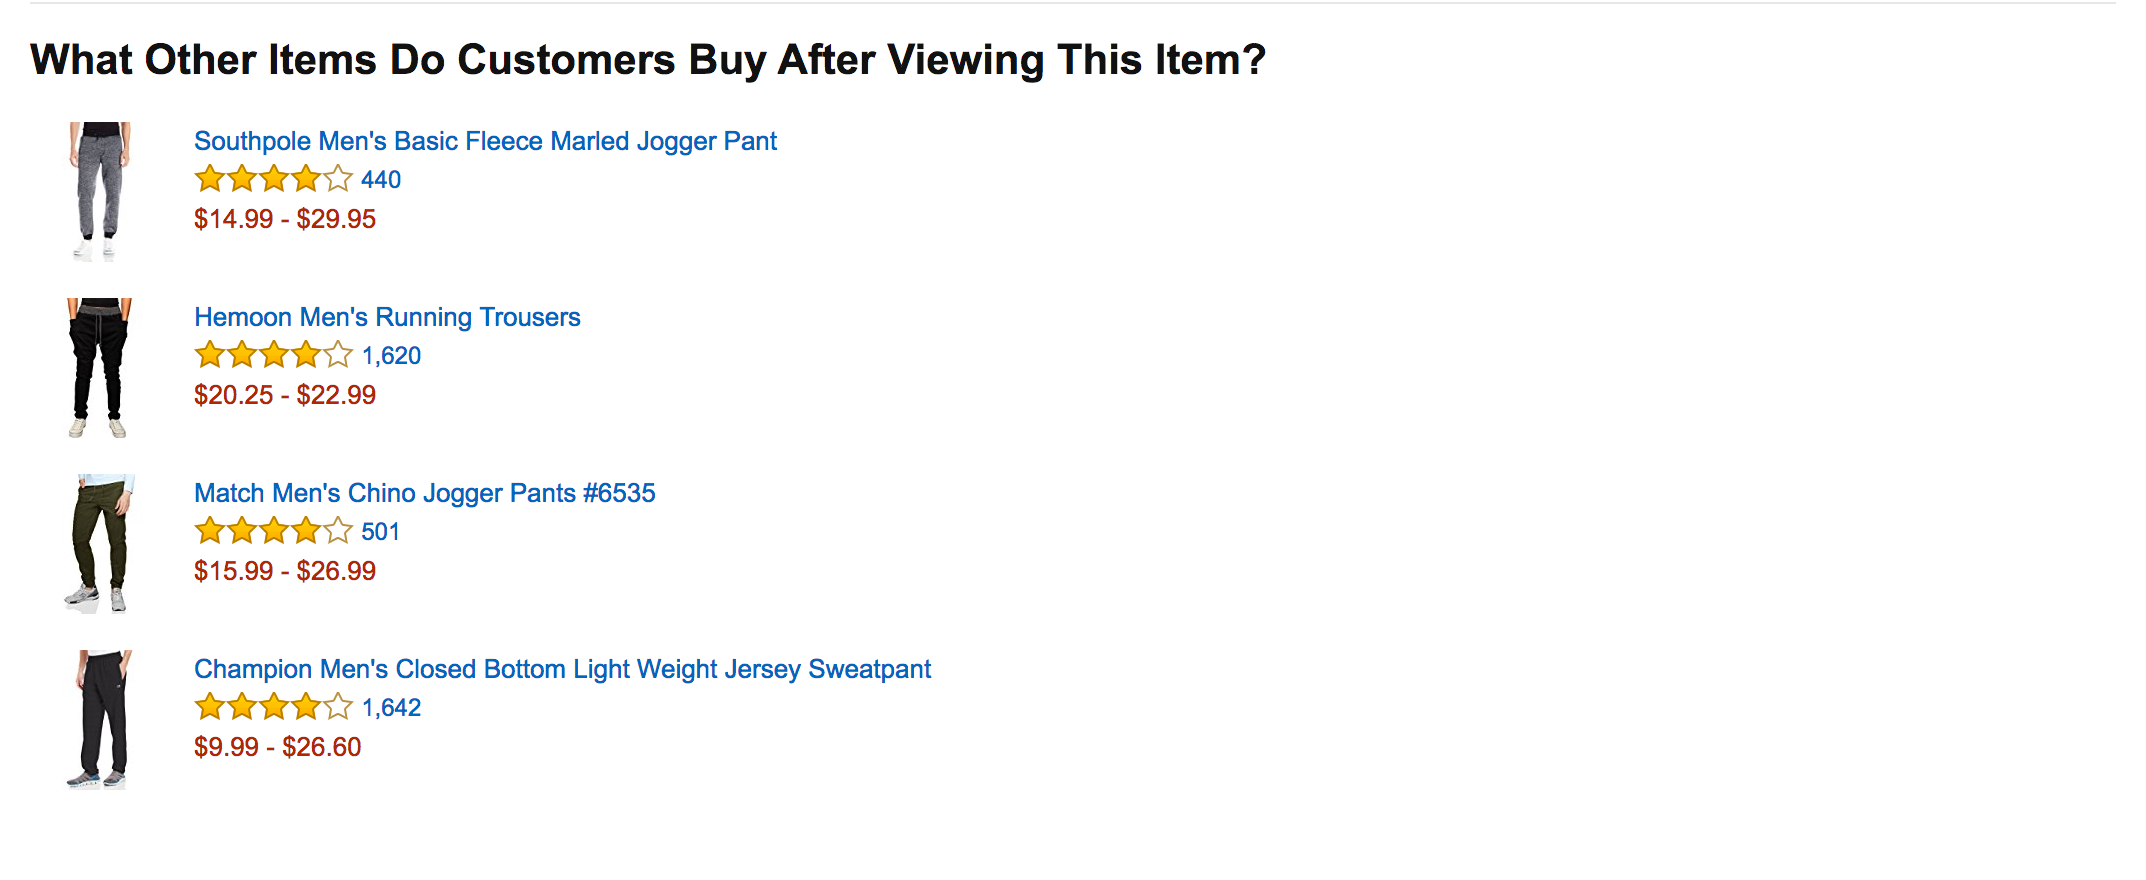
\includegraphics[width=300px,height=300px]{images/sims-consolidated-2_feature_div(2).png}
\caption{(2)}
\end{figure}

\pagebreak

\section*{sims-consolidated-3\_feature\_div}
\begin{figure}[htp]
\centering
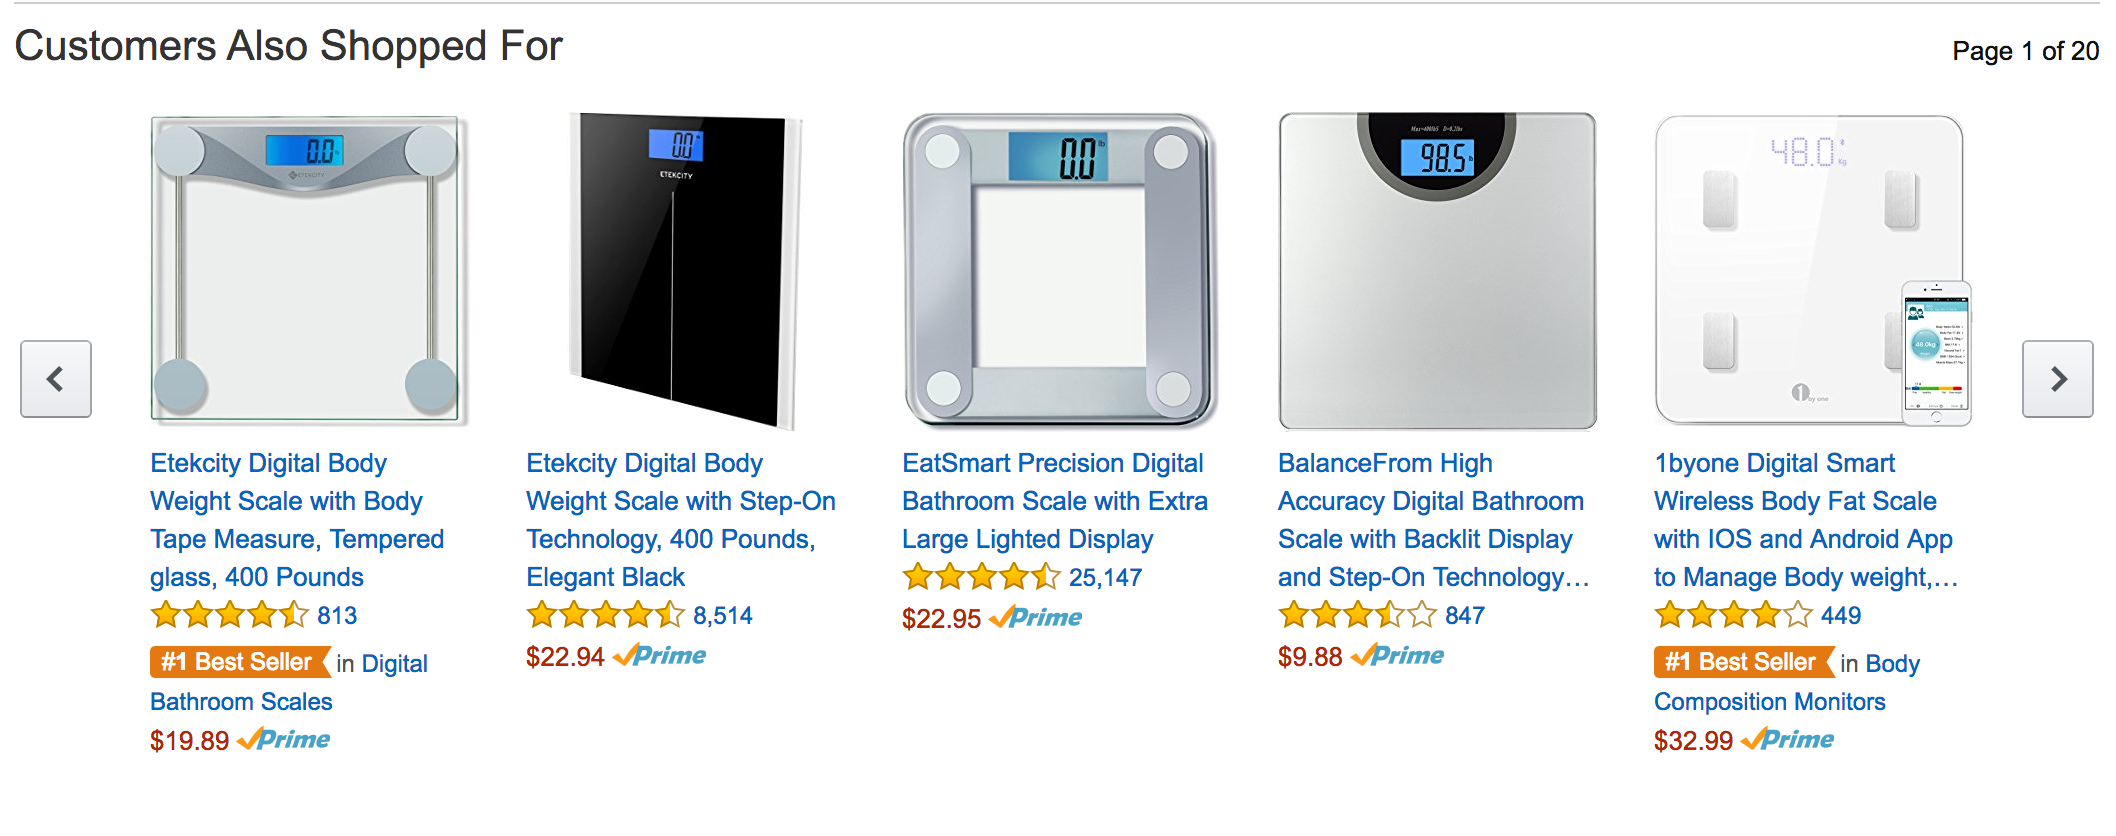
\includegraphics[width=300px,height=300px]{images/sims-consolidated-3_feature_div(1).png}
\caption{(1)}
\end{figure}


\pagebreak

\section*{sponsored-products-dp\_feature\_div}
\begin{figure}[htp]
\centering
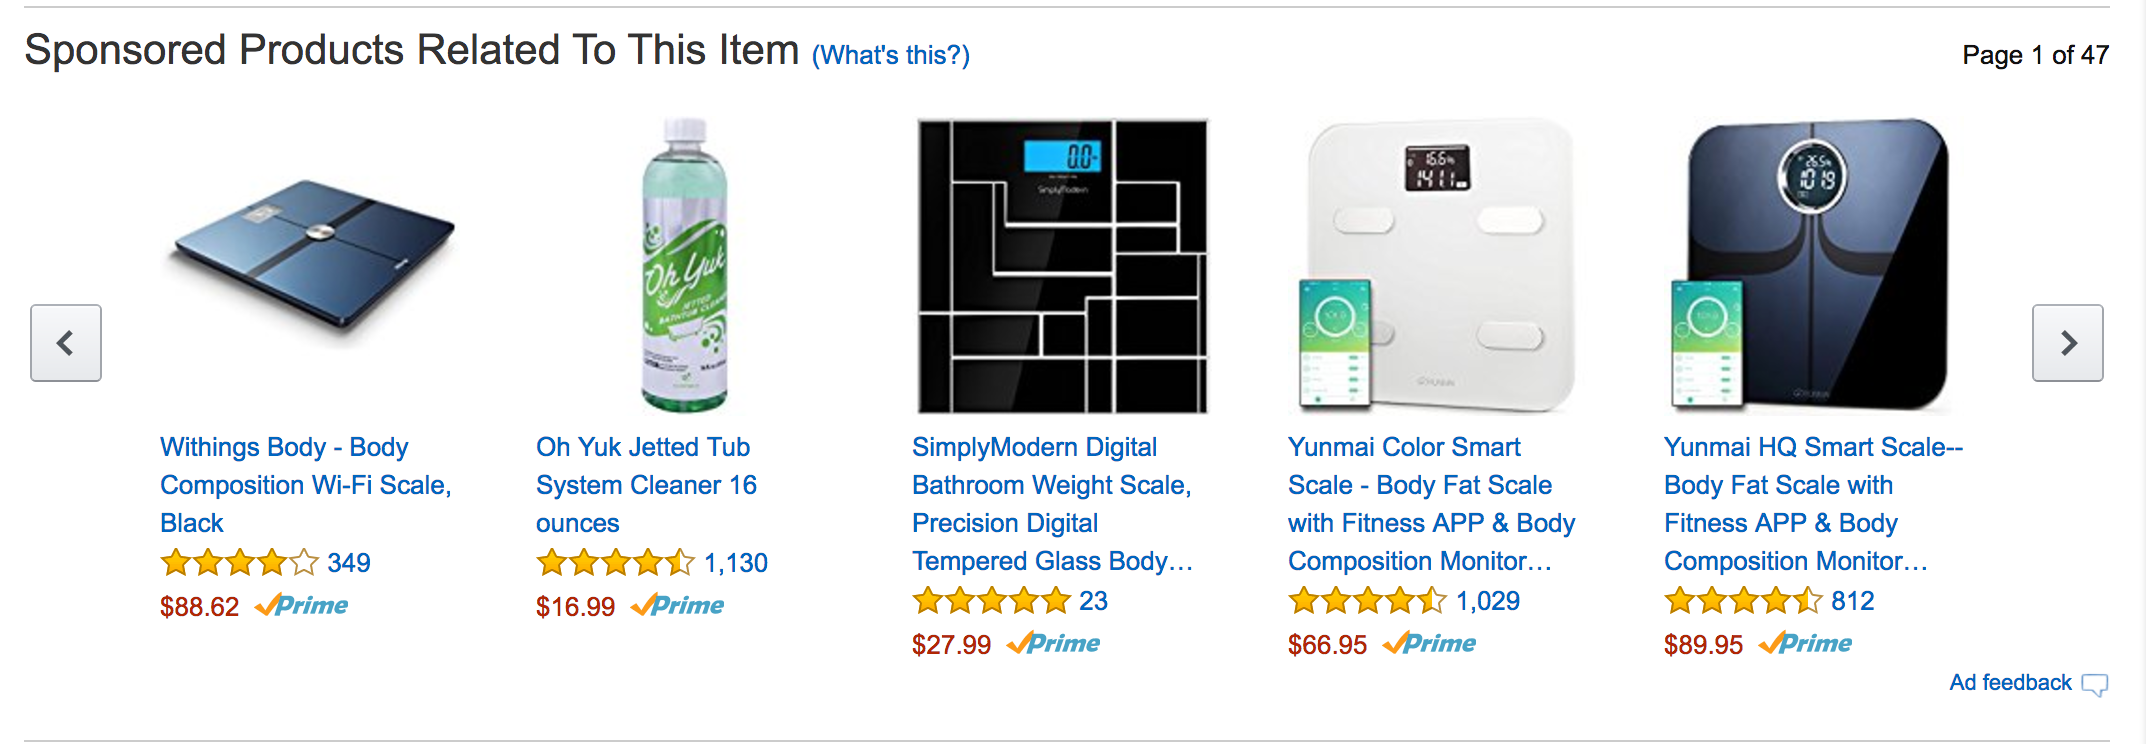
\includegraphics[width=300px,height=300px]{images/sponsored-products-dp_feature_div(1).png}
\caption{(1)}
\end{figure}

\pagebreak

\section*{wayfinding-breadcrumbs\_container}
\begin{figure}[htp]
\centering
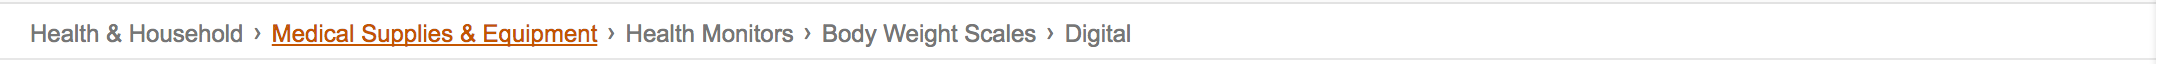
\includegraphics[width=300px,height=300px]{images/wayfinding-breadcrumbs_container(1).png}
\caption{(1)}
\end{figure}

\pagebreak

\begin{figure}[htp]
\centering

\includegraphics[width=300px,height=300px]{images/wayfinding-breadcrumbs_container(2).png}
\caption{(2)}
\end{figure}



\end{document}





















\documentclass[12pt]{article}
\usepackage[english]{babel}
\usepackage{amsmath,amsthm,amsfonts,amssymb,epsfig}
\usepackage[left=.5in,top=.5in,right=.5in, bottom=1in]{geometry}
\usepackage{mathtools}
\usepackage{breqn}



\usepackage{titlesec}
\usepackage{verbatim}
\usepackage{amssymb}
\usepackage{amsmath}
\usepackage{amsthm}
\usepackage{mathrsfs}
\usepackage{enumitem}

\usepackage{graphicx}

%% commands for math note taking 
\newcommand{\defn} [0]  {\paragraph{DEFN : }}
\newcommand{\fact}[0] {\paragraph{FACT : }}
\newcommand{\prop} [0] {\paragraph{PROP  : }}
\newcommand{\thm}[0] {\paragraph{THM : }}
\newcommand{\cor}[0] {\paragraph{COROLLARY : }}
\newcommand{\pf}[0] {\paragraph*{PROOF :}}
\newcommand{\note}[0] {\paragraph*{NOTE :}}
\newcommand{\lemma}[0]{\paragraph*{LEMMA : }}
\DeclarePairedDelimiter{\abs}{\lvert}{\rvert}


\newcommand*{\backnotin}{\rotatebox[origin=c]{-180}{$\notin$}}%

\titleformat{\subsection}{\centering\large\bfseries}{\thesection}{1em}{}



\DeclareMathOperator{\tr}{tr}
\DeclareMathOperator{\im}{im}
\DeclareMathOperator{\Perm}{Perm}
\DeclareMathOperator{\lcm}{lcm}
\DeclareMathOperator{\Var}{Var}
\DeclareMathOperator{\Cov}{Cov}

\title{Amazon HTML Notes}
\author{Darek Johnson}
\date{Mar 4, 2017}

\begin{document}

%%  eliminates page numbers
%%  \pagestyle{empty}

\maketitle

\section*{ }





\end{document}





















